\reportchapter{V. KẾT QUẢ ĐẠT ĐƯỢC VÀ HƯỚNG PHÁT TRIỂN TIẾP THEO}
\reportsection{a. Kết quả đạt được}
Sau khi hoàn thành quá trình phát triển và triển khai, Philobiblus đạt được ba nhóm kết quả chính: giao diện web có thể truy cập, pipeline recommendation được kết nối với dữ liệu và model, và hệ thống được vận hành trên GKE cùng các dịch vụ Google Cloud. Các minh chứng dưới đây được chụp từ phiên bản đang chạy của hệ thống.

Mã nguồn của hệ thống được lưu tại \href{https://github.com/kazunguyen/philobiblus}{repository Philobiblus trên GitHub}. Phiên bản web dùng thử được phát hành tại \href{https://kazunguyen.github.io/philobiblus/}{địa chỉ GitHub Pages của dự án}.

\textbf{Kết quả giao diện và gợi ý sách.} Ở trang thư viện, khu vực \textit{For you} sử dụng các đầu sách người dùng đã đọc làm tín hiệu đầu vào. Recommendation service phân tích metadata của những sách đó, sau đó trả về danh sách các sách có nội dung tương đồng để hiển thị trên giao diện.

\begin{figure}[H]
\centering
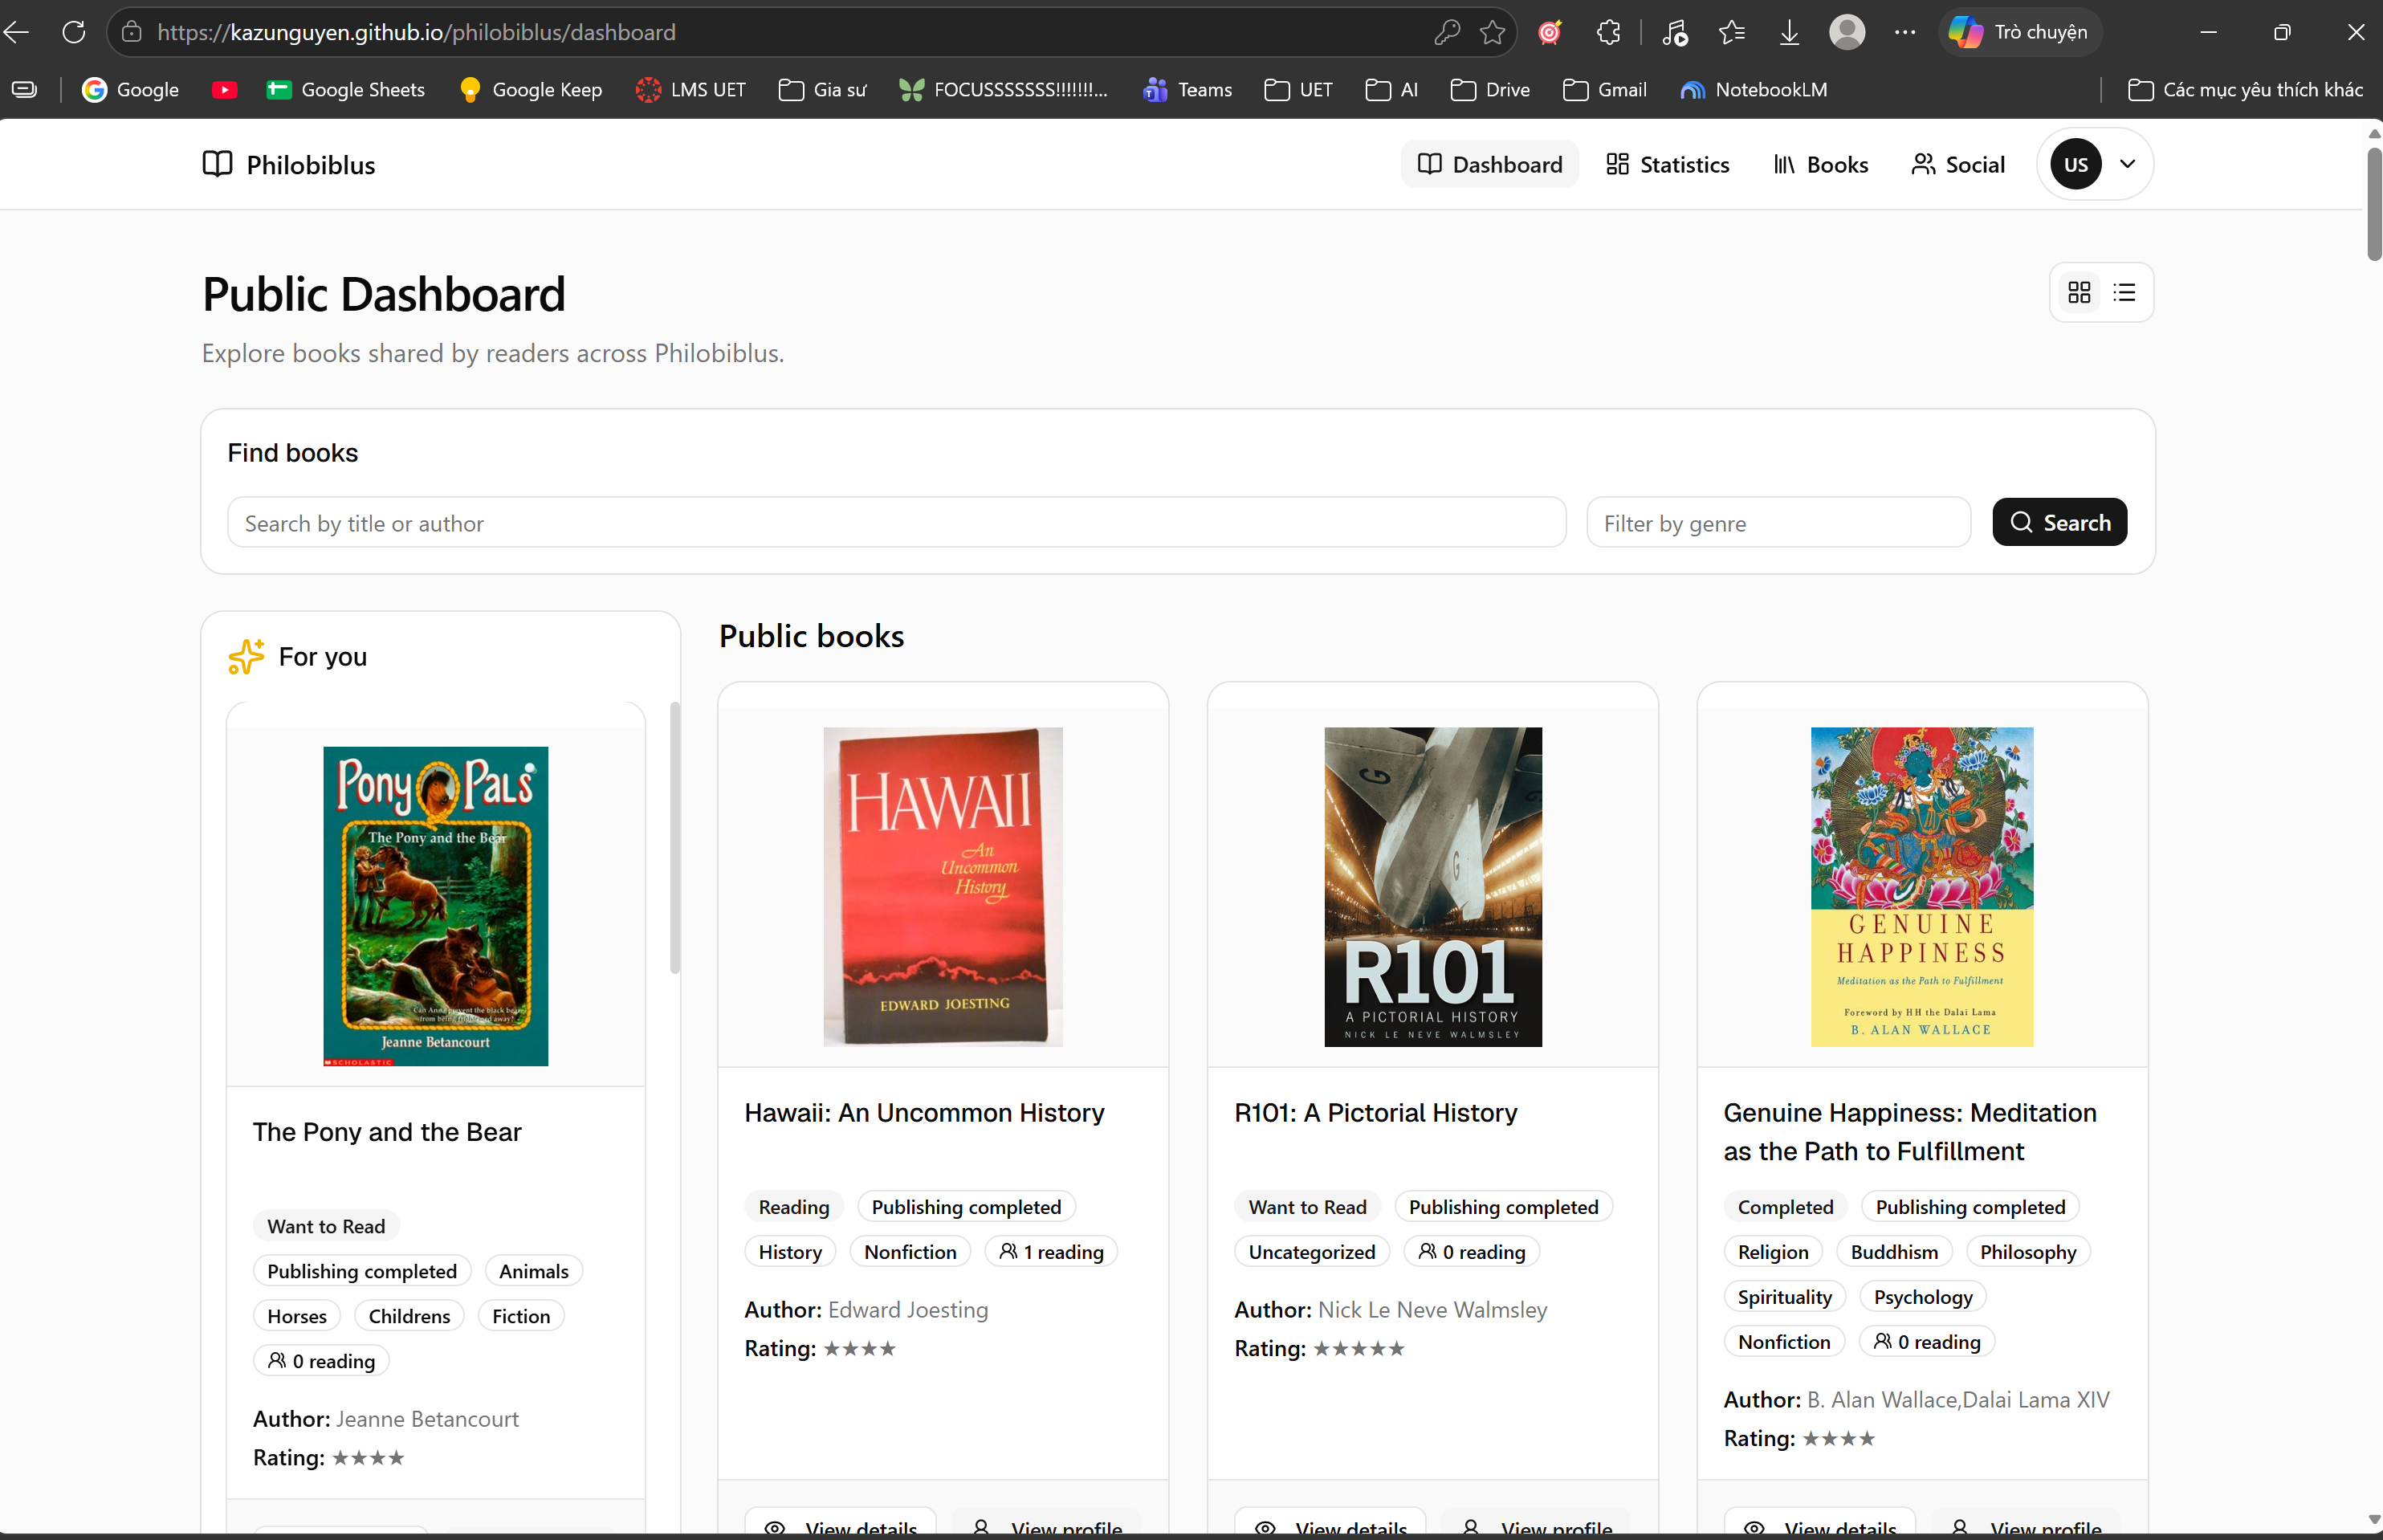
\includegraphics[width=0.94\textwidth]{../../screenshots/11-ui-public-catalog.png}
\caption{Khu vực \textit{For you} hiển thị gợi ý dựa trên lịch sử đọc của người dùng}
\label{fig:for-you-recommendation}
\end{figure}

Khi người dùng mở trang chi tiết một cuốn sách, hệ thống dùng chính cuốn sách đang xem làm sách nguồn. Các metadata của sách nguồn được đưa vào bộ xếp hạng để tìm và hiển thị những đầu sách liên quan, giúp người dùng tiếp tục khám phá nội dung cùng chủ đề.

\begin{figure}[H]
\centering
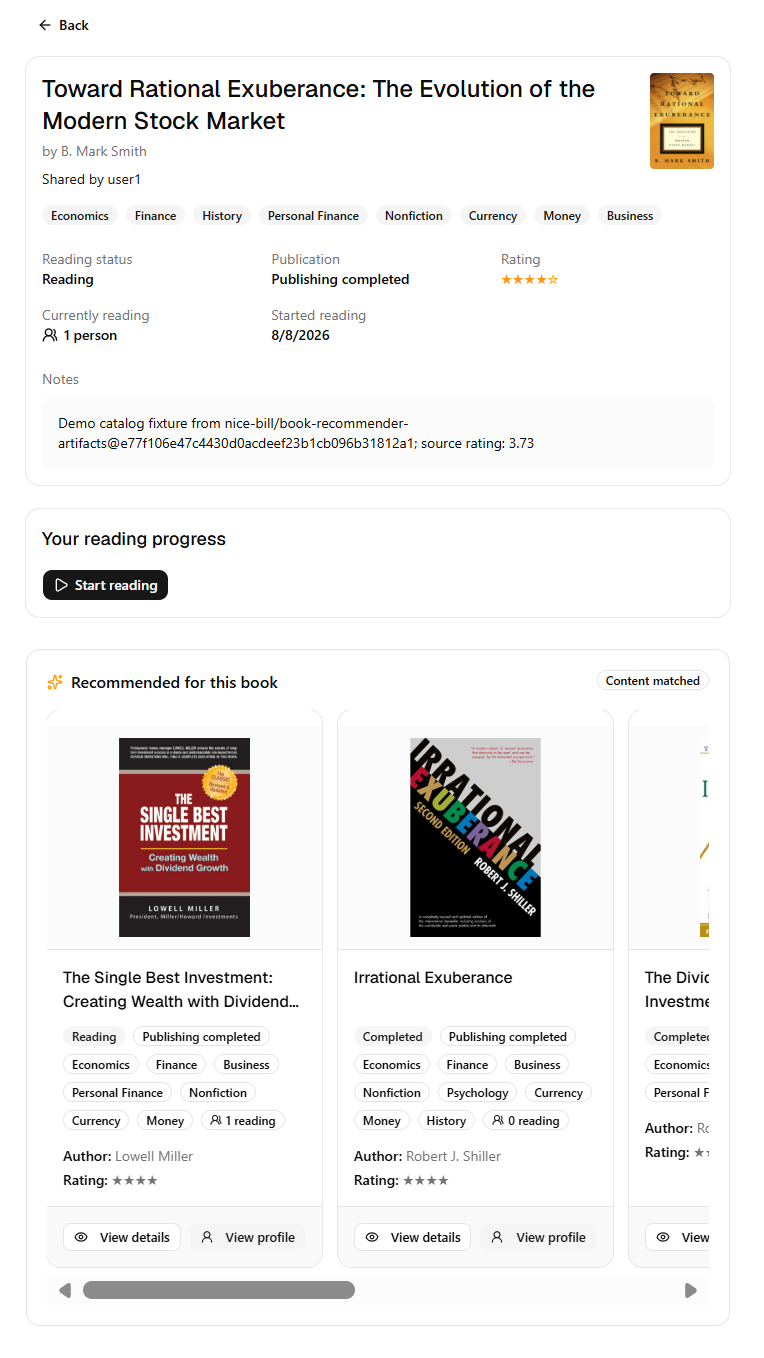
\includegraphics[width=0.82\textwidth]{../../screenshots/book-detail-with-recommendation.png}
\caption{Gợi ý sách liên quan trên trang chi tiết của một cuốn sách}
\label{fig:book-detail-recommendation}
\end{figure}

\textbf{Kết quả triển khai và vận hành.} Các workload phục vụ người dùng và MLOps được tách trong hai namespace của cùng một cụm GKE. Ảnh chụp dưới đây xác nhận các workload đã được tạo và đang được quan sát trên GKE Console.

\begin{figure}[H]
\centering
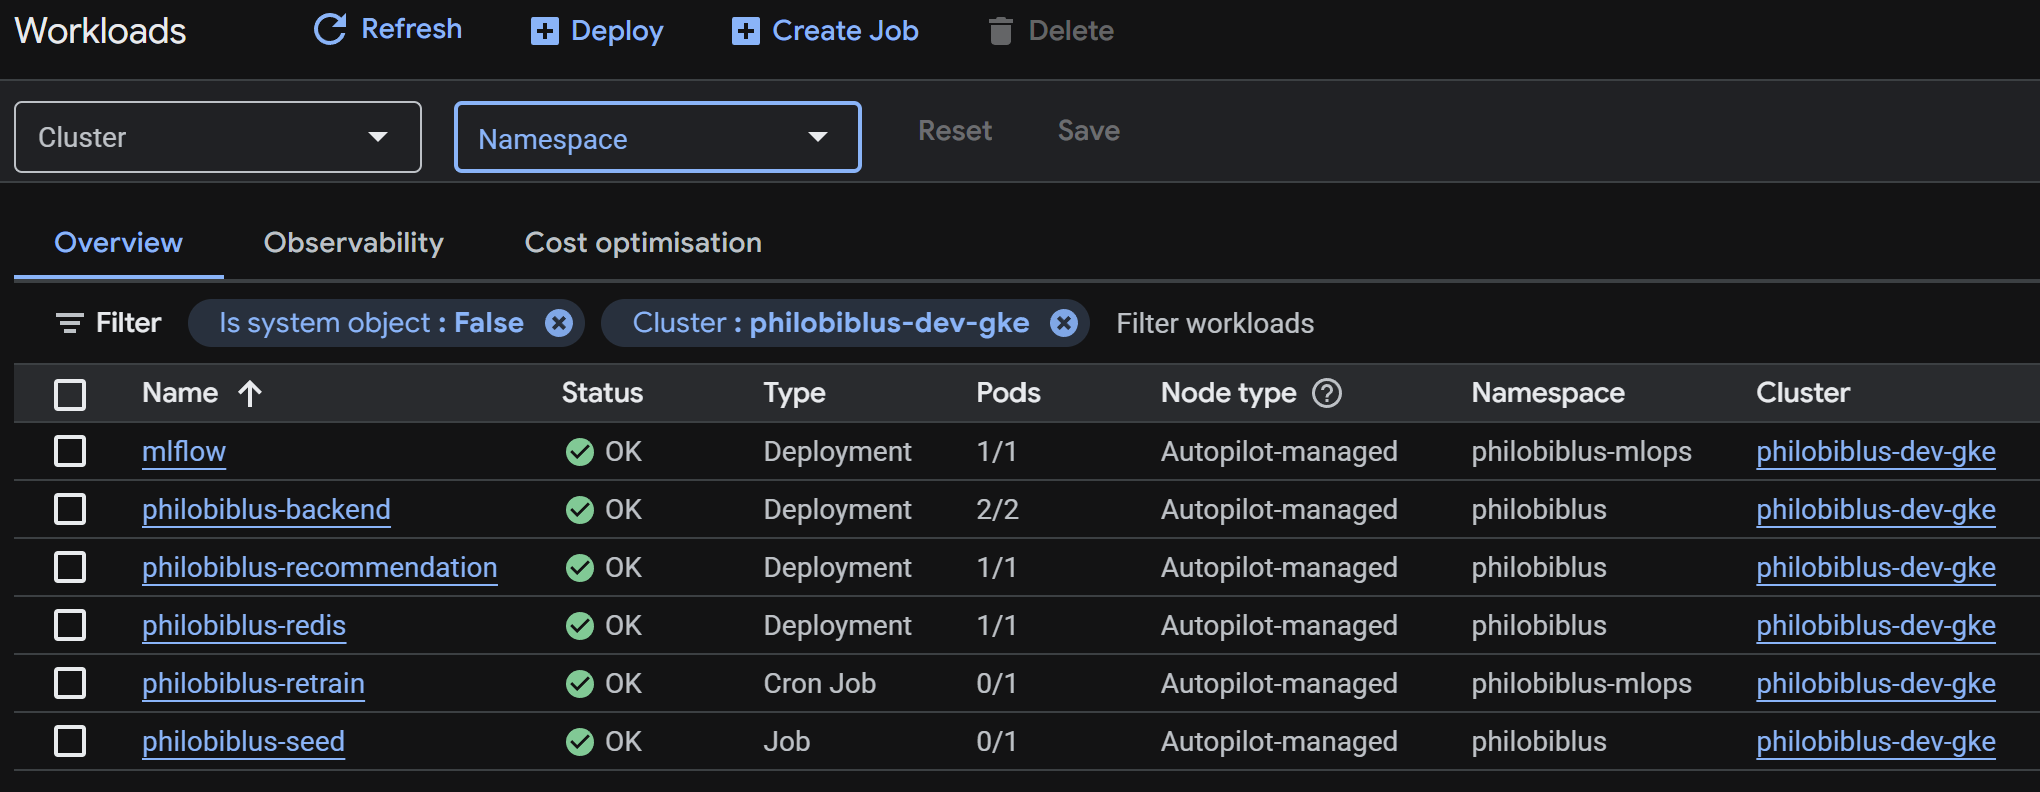
\includegraphics[width=0.47\textwidth]{../../screenshots/02-gke-workloads-philobiblus.png}
\caption{Workload Philobiblus và MLOps quan sát trên GKE Console}
\label{fig:gke-workloads}
\end{figure}

Tại thời điểm ngày 04/10/2026, cluster \texttt{philobiblus-dev-gke} đang chạy ổn định, các tài nguyên chính phục vụ ứng dụng và MLOps đã được triển khai. Hình dưới đây đối chiếu trực tiếp trạng thái của GKE, Cloud SQL, Artifact Registry và Cloud Storage trên Google Cloud Console.

\begin{figure}[H]
\centering
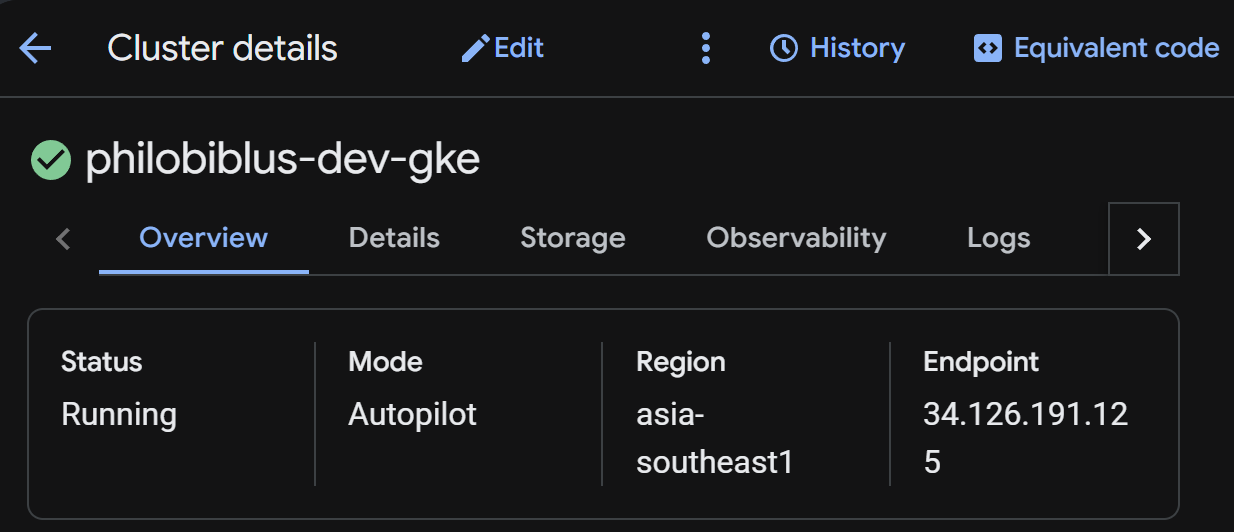
\includegraphics[width=0.47\textwidth]{../../screenshots/01-gke-cluster-overview.png}\hfill
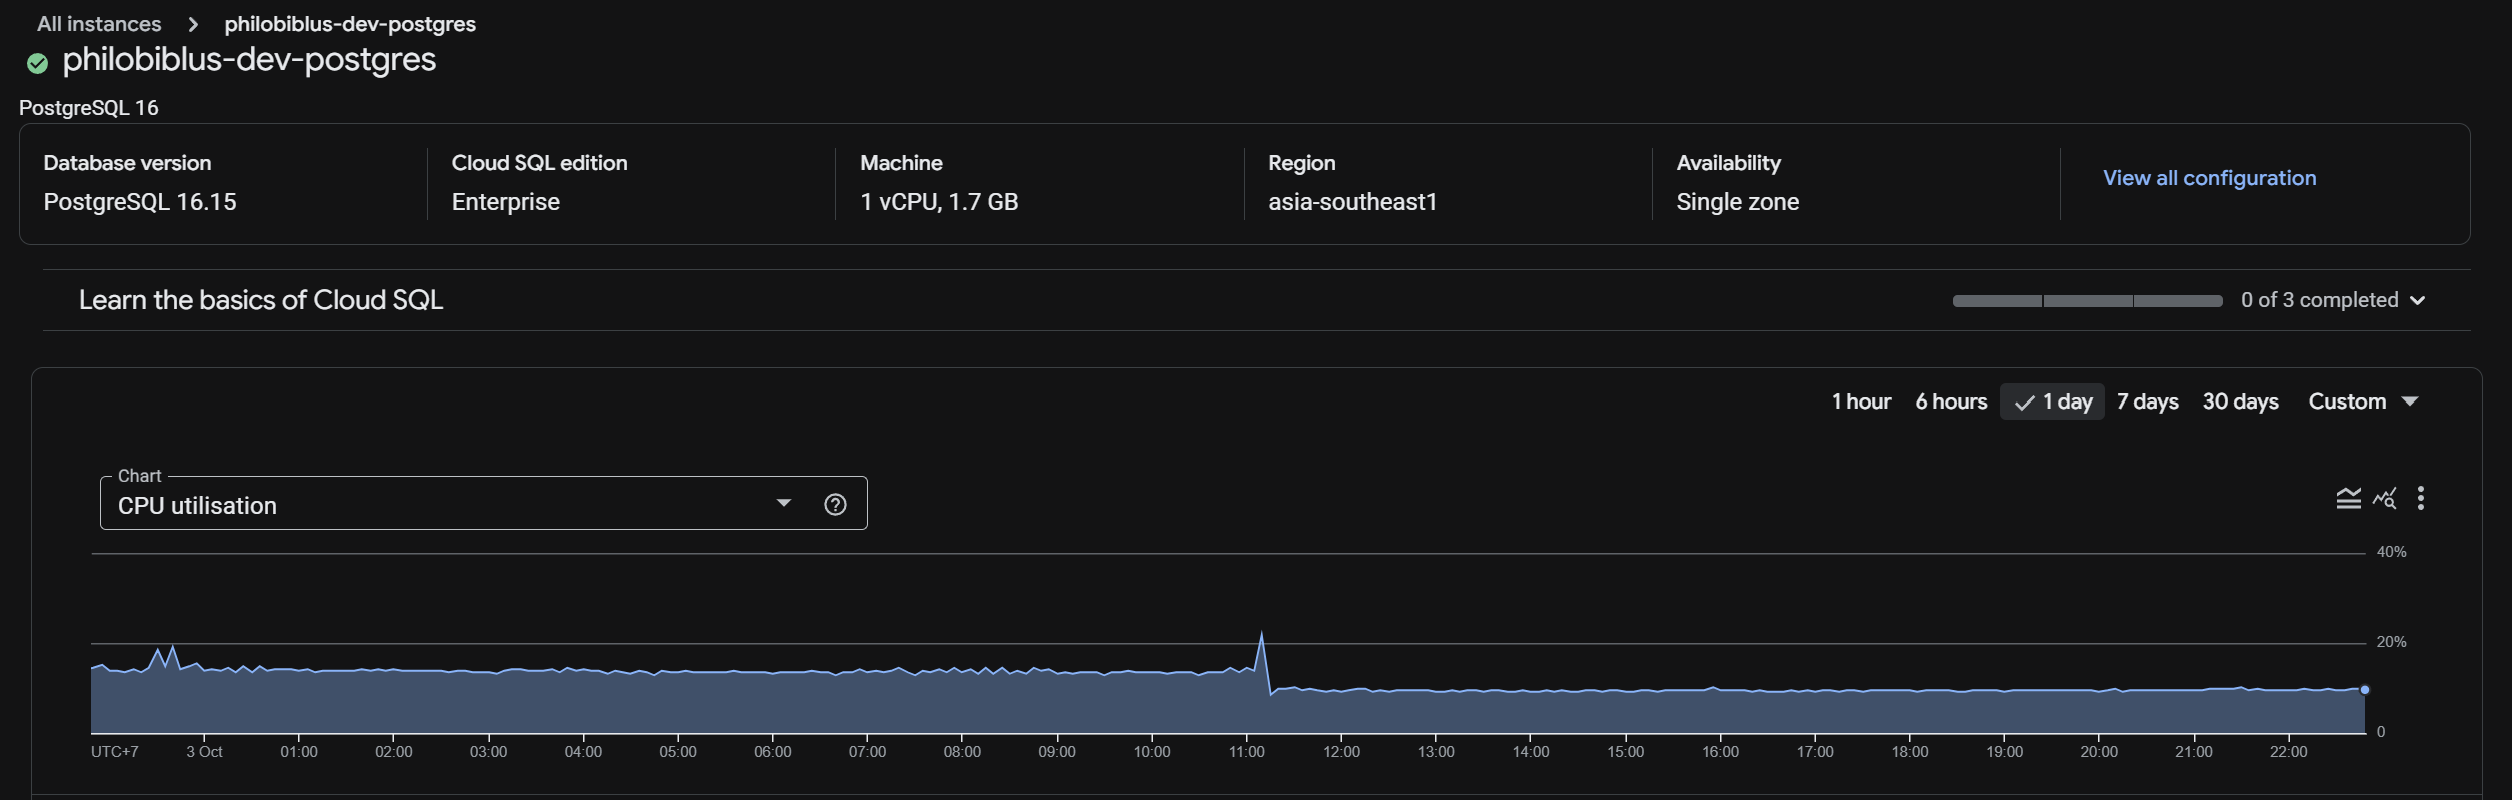
\includegraphics[width=0.47\textwidth]{../../screenshots/06-cloud-sql-overview.png}\\[0.35em]
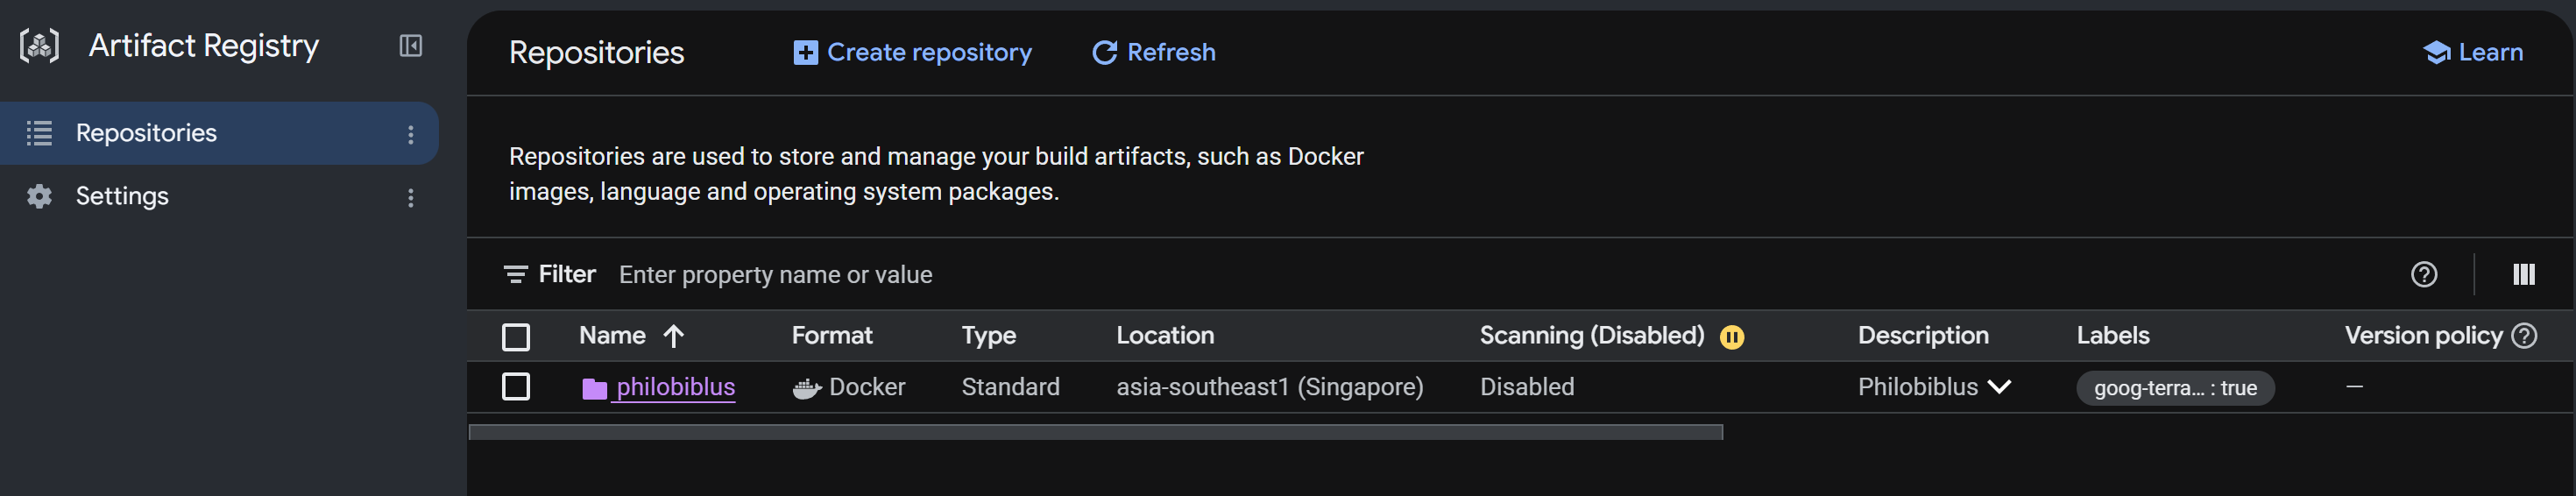
\includegraphics[width=0.47\textwidth]{../../screenshots/gcloud-artifact-registry.png}\hfill
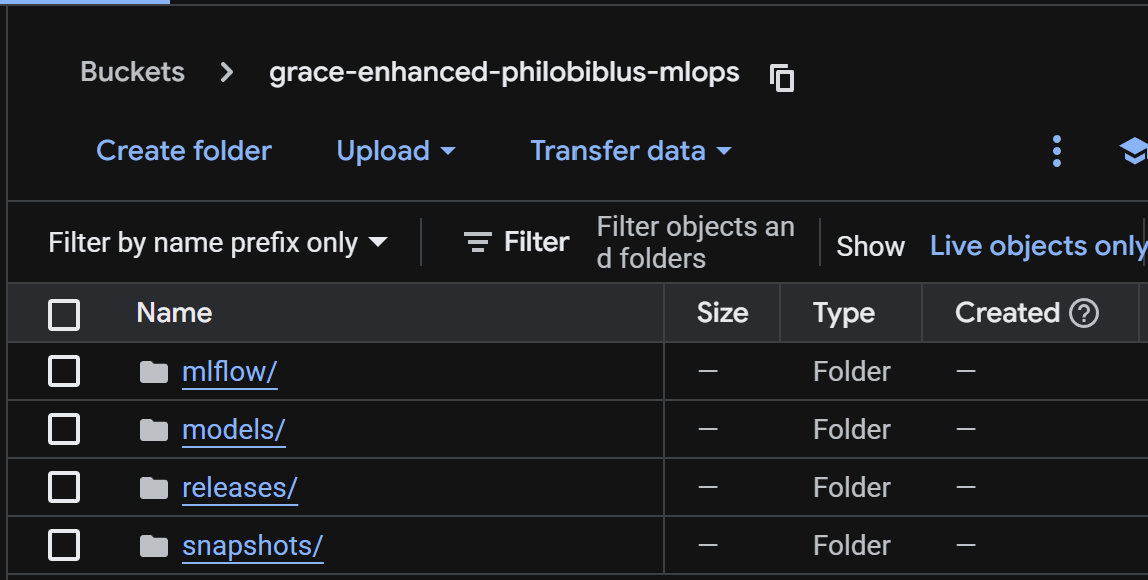
\includegraphics[width=0.47\textwidth]{../../screenshots/09-gcs-mlops-artifacts.png}
\caption{Trạng thái hoạt động của các tài nguyên Google Cloud: GKE, Cloud SQL, Artifact Registry và Cloud Storage}
\label{fig:gcp-runtime-evidence}
\end{figure}

\reportsubsection{Kiểm thử và xác minh}
Các ca kiểm thử được thực hiện trên trạng thái source hiện tại ngày 04/10/2026. Backend và ML chạy trong môi trường Python tạm với dependency lấy từ file \texttt{requirements}; build frontend dùng fixture tương đương GitHub Pages; Helm dùng fixture không chứa secret như workflow CI.

\begin{table}[H]
\centering
\small
\renewcommand{\arraystretch}{1.2}
\begin{tabularx}{\textwidth}{>{\raggedright\arraybackslash}p{1.1cm} >{\raggedright\arraybackslash}p{6.1cm} >{\raggedright\arraybackslash}X}
\toprule
Mã & Ca kiểm thử và phạm vi & Kết quả \\
\midrule
TC-01 & Backend pytest: API nghiệp vụ, JWT và phân quyền, cache catalog, rate limit, observability, recommendation và load shedding. & 63/63 đạt trong 60,03 giây; 2 cảnh báo deprecation từ dependency. \\
TC-02 & ML pytest: recommendation service, TF-IDF recommender, quality gate và snapshot validation. & 17/17 đạt trong 6,89 giây; 1 cảnh báo deprecation từ Starlette. \\
TC-03 & Frontend build Vite với biến môi trường tương đương workflow GitHub Pages. & Thành công: 2.105 module được bundle trong 8,27 giây. \\
TC-04 & Lint và render chart \texttt{philobiblus} và \texttt{philobiblus-mlops} với fixture không chứa secret. & 2/2 chart thành công; chỉ có khuyến nghị thêm icon cho Chart.yaml. \\
TC-05 & Truy vấn chỉ đọc trạng thái GKE, Cloud Run, Cloud SQL, Artifact Registry và Cloud Storage. & GKE RUNNING, proxy READY, Cloud SQL RUNNABLE; repository và bucket MLOps tồn tại. \\
\bottomrule
\end{tabularx}
\caption{Kết quả kiểm thử và xác minh triển khai}
\label{tab:test-results}
\end{table}

Backend pytest dùng SQLite in-memory để cô lập test API, nên không thay thế kiểm thử tích hợp với Cloud SQL. Helm lint và template kiểm tra tính hợp lệ của manifest trước triển khai, không thay thế việc rollout trên cluster. Hai giới hạn này được giữ tách biệt với kết quả xác minh resource GCP để tránh diễn giải quá mức phạm vi kiểm thử.

\reportsubsection{Kiểm thử tải}
Lần kiểm tra đầu đạt 120 người dùng đồng thời với 23,4 request/giây, p95 322,5 ms và 0,94 phần trăm lỗi; tại 125 người dùng, lỗi tăng lên 1,48 phần trăm. Sau khi thêm Redis cache TTL 30 giây và giới hạn pool 3 + overflow 2 cho mỗi Pod, mốc 150 người dùng đạt 29,6 request/giây, p95 138,6 ms và không có request lỗi.

\clearpage
\begin{figure}[H]
\centering
\includegraphics[width=0.94\textwidth]{capacity-comparison.png}
\caption{Độ trễ và tỷ lệ lỗi tại các mốc tải chung trước và sau tối ưu}
\label{fig:6}
\end{figure}
150 người dùng là mốc cao nhất đã kiểm tra; ở lần benchmark này recommendation service được tắt để cô lập backend cùng database. Vì vậy kết quả không đại diện cho năng lực khi đồng thời phục vụ workload gợi ý. Môi trường dev hiện bật recommendation service và dùng circuit breaker Redis chung: vượt 12 request trong 10 giây thì API trả unavailable trong 30 giây, sau đó tự phục hồi. Mức vận hành đề xuất vẫn là 120 đến 130 người dùng đồng thời, khoảng 24 request/giây, trước khi thực hiện lần đo đầy đủ hơn có recommendation service.

Đối chiếu với các yêu cầu tại Chương II, Philobiblus đã đáp ứng các luồng chức năng cốt lõi gồm quản lý tài khoản, thư viện, tiến độ đọc, tương tác, chia sẻ và gợi ý sách. Các yêu cầu phi chức năng về bảo mật, triển khai lặp lại, mở rộng, MLOps, quan sát và kiểm thử đã được áp dụng ở mức phù hợp với phạm vi thực tập; một số giới hạn còn lại nằm ở chất lượng mô hình, kiểm thử tích hợp, rollback và quy trình CD production.

\reportsection{b. Kỹ năng và kiến thức thu thập được}
Trong kỳ thực tập, em đã được thực hành theo dõi toàn bộ hệ thống từ mã nguồn, kiểm thử và image đến Terraform, Helm, GKE và quan sát vận hành, nhờ đó em có thể hiểu rõ hơn cách Service, probe, resource, secret, policy mạng và rollout phối hợp trong một workload thực tế. Ngoài ra, nhờ được thực hành quản lý snapshot, artifact, quality gate, JWT, quyền sở hữu, Cloud Armor, NetworkPolicy và kiểm tra chuỗi cung ứng phần mềm, em đã củng cố kiến thức về DevOps, MLOps và DevSecOps, đồng thời rèn luyện kỹ năng lập trình, kiểm thử, triển khai và vận hành hệ thống cho mình.

\reportsection{d. Hướng phát triển tiếp theo để hoàn thiện giải pháp}
Kết quả benchmark cho em thấy khá rõ giới hạn của cấu hình hiện tại: hệ thống phù hợp hơn với khoảng 120 đến 130 người dùng đồng thời, còn mốc 150 người dùng mới chỉ được đo khi tắt recommendation service. Nếu tiếp tục phát triển, em sẽ phải đánh giá lại toàn bộ luồng, bao gồm cả nghiệp vụ và recommendation, thay vì chỉ nhìn vào kết quả benchmark đã cô lập backend với cơ sở dữ liệu. Những giới hạn về cache, connection pool và năng lực Cloud SQL sẽ là dữ liệu đầu vào để lựa chọn cách phân vùng tải và chính sách autoscaling ở các giai đoạn sau.

Ở giai đoạn sau, hệ thống sẽ cần chuyển Cloud Armor từ chế độ preview sang enforce, xác minh nguồn gốc artifact bằng chữ ký và nối trace, PolicyReport, log với cảnh báo trong cùng một quy trình xử lý sự cố. Còn đối với chức năng gợi ý sách, em muốn tiếp tục thu thập thêm lịch sử đọc để đánh giá mô hình trên dữ liệu thực tế hơn. Sau khi có đủ dữ liệu, em sẽ train model gợi ý mới kết hợp thông tin nội dung với hành vi người dùng để cải thiện chất lượng gợi ý.
